% ex: ts=2 sw=2 sts=2 et filetype=tex
% SPDX-License-Identifier: CC-BY-SA-4.0

\documentclass[10pt,addpoints]{exam}

\usepackage[utf8]{inputenc}
\usepackage[T1]{fontenc}
\usepackage[letterpaper]{geometry}
\usepackage{graphicx}
\usepackage{xcolor}
%\usepackage[spanish]{babel}

\definecolor{itesoprofundo}{RGB}{000, 066, 112}
\definecolor{itesomedio}{RGB}{112, 144, 183}
\definecolor{itesoclaro}{RGB}{151, 227, 255}

\pagestyle{headandfoot}
%\headrule
\lhead{\includegraphics[scale=0.5]{logo.png}}{}
\rhead{\color{itesoprofundo}\textbf{ALGORITMOS Y PROGRAMACIÓN}\\Departamento
       de Electrónica, Sistemas e Informática\\}
\footer{}{Página \thepage\ de \numpages}{}

\pointpoints{punto}{puntos}
\renewcommand{\solutiontitle}{\textbf{Solución: }}

%\printanswers

\begin{document}
\begin{center}
  \sffamily\textbf{EXAMEN I}
\end{center}
\begin{flushright}
8 de octubre de 2023
\end{flushright}
Nombre:~\makebox[4in]{\hrulefill}
Puntos máximos: 100

\begin{questions}

\begin{EnvFullwidth}
  \sffamily\textbf{Sección I.- Completar los siguientes enunciados con las
  palabras situadas en la parte inferior de la sección (valor 15 puntos).}
\end{EnvFullwidth}

% ex: ts=2 sw=2 sts=2 et filetype=tex
% SPDX-License-Identifier: CC-BY-SA-4.0

\question Esta dada por la correspondencia entre los elementos de dos
          conjuntos que forman parejas ordenadas, la formulación de una
          expresión que une dos o mas objetos entre si establece una \fillin

  \begin{oneparchoices}
    \choice función
    \CorrectChoice relación
    \choice correspondencia
  \end{oneparchoices}

% ex: ts=2 sw=2 sts=2 et filetype=tex
% SPDX-License-Identifier: CC-BY-SA-4.0

\question Es el conjunto donde la función esa definida, osea donde puede
tomar sus valores y realizar las operaciones qu se indican en  dicha
relación.


  \begin{oneparchoices}
    \choice Función
    \choice Dominio
    \choice Contradominio
    \choice Cuadratica
  \end{oneparchoices}
  %\answerline[A]

% ex: ts=2 sw=2 sts=2 et filetype=tex
% SPDX-License-Identifier: CC-BY-SA-4.0

\question A partir del Teorema de \fillin \enspace podemos encontrar la
          distancia entre dos puntos.

  \begin{oneparchoices}
    \choice Distancia de puntos
    \choice $c^2 = a^3 + b^4$
    \CorrectChoice Pitagoras
    \choice Los ángulos
  \end{oneparchoices}
  \answerline[C]

% ex: ts=2 sw=2 sts=2 et filetype=tex
% SPDX-License-Identifier: CC-BY-SA-4.0

\question Clasifica las siguientes funciones:

\begin{parts}
  \part $y=3^{4x-1}$
  \part $y=\sqrt[3]{8x^2-x+10}$
  \part $f(x)=sen(4x-9)$
\end{parts}


% ex: ts=2 sw=2 sts=2 et filetype=tex
% SPDX-License-Identifier: CC-BY-SA-4.0

\question Usa la siguiente cuadricula para resolver los siguientes incisos:

  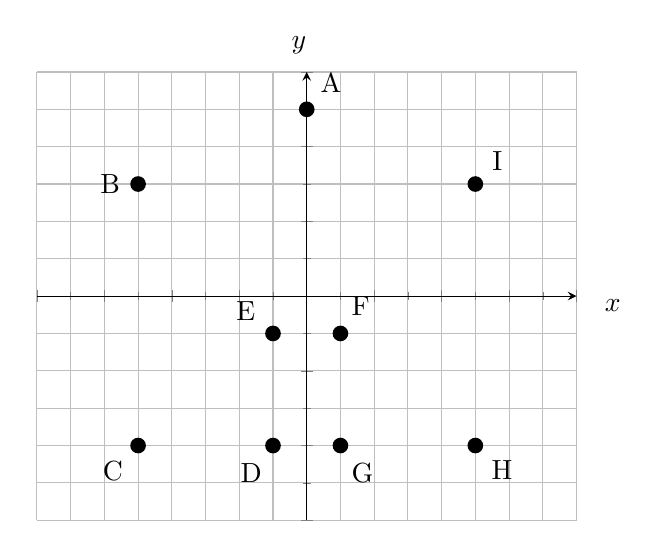
\begin{tikzpicture}
    \begin{axis}[grid=both,ymin=-6,ymax=6,xmax=8,xmin=-8,xticklabel=\empty,yticklabel=\empty,
               minor tick num=1,axis lines = middle,xlabel=$x$,ylabel=$y$,
               label style = {at={(ticklabel cs:1.1)}}]
      \node[label={60:{A}},circle,fill,inner sep=2pt] at (axis cs:0,5) {};
      \node[label={180:{B}},circle,fill,inner sep=2pt] at (axis cs:-5,3) {};
      \node[label={30:{I}},circle,fill,inner sep=2pt] at (axis cs:5,3) {};
      \node[label={230:{C}},circle,fill,inner sep=2pt] at (axis cs:-5,-4) {};
      \node[label={320:{H}},circle,fill,inner sep=2pt] at (axis cs:5,-4) {};
      \node[label={160:{E}},circle,fill,inner sep=2pt] at (axis cs:-1,-1) {};
      \node[label={80:{F}},circle,fill,inner sep=2pt] at (axis cs:1,-1) {};
      \node[label={260:{D}},circle,fill,inner sep=2pt] at (axis cs:-1,-4) {};
      \node[label={280:{G}},circle,fill,inner sep=2pt] at (axis cs:1,-4) {};
    \end{axis}
  \end{tikzpicture}

  \begin{parts}
    \part Encuantra las coordenadas de los vértices en el polígono. \\
    A(\fillin\ ,\fillin\ ) \enspace B(\fillin\ ,\fillin\ ) \\
    C(\fillin\ ,\fillin\ ) \enspace D(\fillin\ ,\fillin\ ) \\
    E(\fillin\ ,\fillin\ ) \enspace F(\fillin\ ,\fillin\ ) \\
    G(\fillin\ ,\fillin\ ) \enspace H(\fillin\ ,\fillin\ ) \\
    I(\fillin\ ,\fillin\ ) \\
    \part Determina el cuadrante en el que se ubica los puntos: \\
    El punto B esta en el cuadrante:\fillin \\
    El punto C esta en el cuadrante:\fillin \\
    El punto D esta en el cuadrante:\fillin \\
    El punto E esta en el cuadrante:\fillin \\
    El punto F esta en el cuadrante:\fillin \\
    El punto G esta en el cuadrante:\fillin \\
    El punto H esta en el cuadrante:\fillin \\
    El punto I esta en el cuadrante:\fillin \\
    \part Sacar la distancia entre los puntos: \\
    AB \fillin \enspace BC \fillin \enspace CD \fillin \enspace DE \fillin \enspace \\
    EF \fillin \enspace FG \fillin \enspace GH \fillin \enspace HI \fillin \enspace  \\
    IA \fillin \enspace
    \part Calcula el perímetro de la figura resultante.
  \end{parts}

% ex: ts=2 sw=2 sts=2 et filetype=tex
% SPDX-License-Identifier: CC-BY-SA-4.0

\question Un \fillin \enspace  es un programa que se encarga de traducir el código fuente a un 
código objeto (bytecode), y que junto un enlazador genera un programa en lenguaje 
máquina directamente ejecutable

  \begin{oneparchoices}
    \choice IDE
    \choice lenguaje
    \CorrectChoice compilador
    \choice pseudocódigo
  \end{oneparchoices}

% ex: ts=2 sw=2 sts=2 et filetype=tex
% SPDX-License-Identifier: CC-BY-SA-4.0

\question Escribe a cúal tipo de funciones pertenece cada expresión:

\renewcommand{\labelenumi}{\alph{enumi})} % Usa letras minúsculas en lugar de números
\begin{enumerate}
  \item $f(x) = 4$ \fillin[constante]
  \item $f(x) = 7x - 4$ \fillin[lineal]
  \item $f(x) = x^2 + 2x + 3$ \fillin[cuadrática]
  \item $f(x) = a^x$ \fillin[exponencial]
\end{enumerate}

% ex: ts=2 sw=2 sts=2 et filetype=tex
% SPDX-License-Identifier: CC-BY-SA-4.0

\question ¿Cuál es el alor de f(2) si $f(x) = 3x + 1$?

  \begin{oneparchoices}
    \choice 4
    \choice 6
    \CorrectChoice  7
  \end{oneparchoices}

% ex: ts=2 sw=2 sts=2 et filetype=tex
% SPDX-License-Identifier: CC-BY-SA-4.0

\question \[ \frac{9}{7} \times \frac{3}{2} = \frac{\hspace{2cm}}{\hspace{2cm}} 
             \hspace{2cm}
             \frac{7}{3} \times \frac{4}{6} = \frac{\hspace{2cm}}{\hspace{2cm}}
          \]

% ex: ts=2 sw=2 sts=2 et filetype=tex
% SPDX-License-Identifier: CC-BY-SA-4.0

\question ¿Cómo se escribe en notación cientifica el siguiente valor
  $0.0000982$?

  \begin{oneparchoices}
    \choice $9.82\times10^{-2}$
    \choice $9.82\times10^{-0}$
    \choice $9.82\times10^{3}$
    \CorrectChoice $9.82\times10^{-5}$
  \end{oneparchoices}
  \answerline[D]

% ex: ts=2 sw=2 sts=2 et filetype=tex
% SPDX-License-Identifier: CC-BY-SA-4.0

\question Esta dada por la correspondencia entre los elementos de dos
          conjuntos que forman parejas ordenadas, la formulación de una
          expresión que une dos o mas objetos entre si establece una \fillin

  \begin{oneparchoices}
    \choice función
    \CorrectChoice relación
    \choice correspondencia
  \end{oneparchoices}

% ex: ts=2 sw=2 sts=2 et filetype=tex
% SPDX-License-Identifier: CC-BY-SA-4.0

\question Es el conjunto donde la función esa definida, osea donde puede
tomar sus valores y realizar las operaciones qu se indican en  dicha
relación.


  \begin{oneparchoices}
    \choice Función
    \choice Dominio
    \choice Contradominio
    \choice Cuadratica
  \end{oneparchoices}
  %\answerline[A]

% ex: ts=2 sw=2 sts=2 et filetype=tex
% SPDX-License-Identifier: CC-BY-SA-4.0

\question A partir del Teorema de \fillin \enspace podemos encontrar la
          distancia entre dos puntos.

  \begin{oneparchoices}
    \choice Distancia de puntos
    \choice $c^2 = a^3 + b^4$
    \CorrectChoice Pitagoras
    \choice Los ángulos
  \end{oneparchoices}
  \answerline[C]

% ex: ts=2 sw=2 sts=2 et filetype=tex
% SPDX-License-Identifier: CC-BY-SA-4.0

\question Clasifica las siguientes funciones:

\begin{parts}
  \part $y=3^{4x-1}$
  \part $y=\sqrt[3]{8x^2-x+10}$
  \part $f(x)=sen(4x-9)$
\end{parts}


% ex: ts=2 sw=2 sts=2 et filetype=tex
% SPDX-License-Identifier: CC-BY-SA-4.0

\question Usa la siguiente cuadricula para resolver los siguientes incisos:

  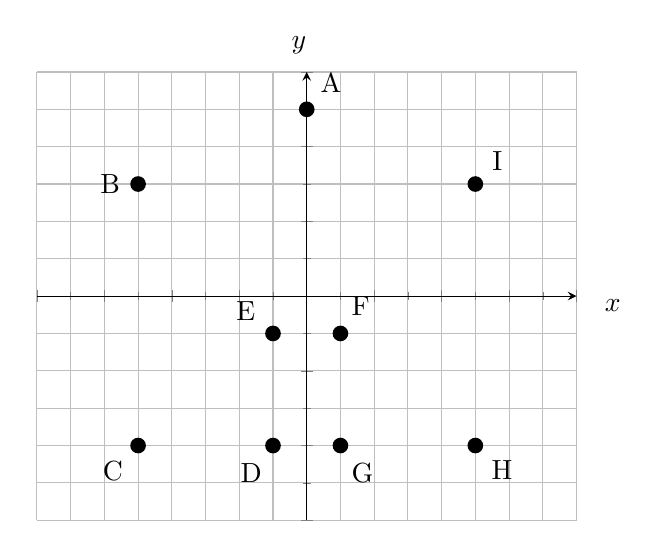
\begin{tikzpicture}
    \begin{axis}[grid=both,ymin=-6,ymax=6,xmax=8,xmin=-8,xticklabel=\empty,yticklabel=\empty,
               minor tick num=1,axis lines = middle,xlabel=$x$,ylabel=$y$,
               label style = {at={(ticklabel cs:1.1)}}]
      \node[label={60:{A}},circle,fill,inner sep=2pt] at (axis cs:0,5) {};
      \node[label={180:{B}},circle,fill,inner sep=2pt] at (axis cs:-5,3) {};
      \node[label={30:{I}},circle,fill,inner sep=2pt] at (axis cs:5,3) {};
      \node[label={230:{C}},circle,fill,inner sep=2pt] at (axis cs:-5,-4) {};
      \node[label={320:{H}},circle,fill,inner sep=2pt] at (axis cs:5,-4) {};
      \node[label={160:{E}},circle,fill,inner sep=2pt] at (axis cs:-1,-1) {};
      \node[label={80:{F}},circle,fill,inner sep=2pt] at (axis cs:1,-1) {};
      \node[label={260:{D}},circle,fill,inner sep=2pt] at (axis cs:-1,-4) {};
      \node[label={280:{G}},circle,fill,inner sep=2pt] at (axis cs:1,-4) {};
    \end{axis}
  \end{tikzpicture}

  \begin{parts}
    \part Encuantra las coordenadas de los vértices en el polígono. \\
    A(\fillin\ ,\fillin\ ) \enspace B(\fillin\ ,\fillin\ ) \\
    C(\fillin\ ,\fillin\ ) \enspace D(\fillin\ ,\fillin\ ) \\
    E(\fillin\ ,\fillin\ ) \enspace F(\fillin\ ,\fillin\ ) \\
    G(\fillin\ ,\fillin\ ) \enspace H(\fillin\ ,\fillin\ ) \\
    I(\fillin\ ,\fillin\ ) \\
    \part Determina el cuadrante en el que se ubica los puntos: \\
    El punto B esta en el cuadrante:\fillin \\
    El punto C esta en el cuadrante:\fillin \\
    El punto D esta en el cuadrante:\fillin \\
    El punto E esta en el cuadrante:\fillin \\
    El punto F esta en el cuadrante:\fillin \\
    El punto G esta en el cuadrante:\fillin \\
    El punto H esta en el cuadrante:\fillin \\
    El punto I esta en el cuadrante:\fillin \\
    \part Sacar la distancia entre los puntos: \\
    AB \fillin \enspace BC \fillin \enspace CD \fillin \enspace DE \fillin \enspace \\
    EF \fillin \enspace FG \fillin \enspace GH \fillin \enspace HI \fillin \enspace  \\
    IA \fillin \enspace
    \part Calcula el perímetro de la figura resultante.
  \end{parts}

% ex: ts=2 sw=2 sts=2 et filetype=tex
% SPDX-License-Identifier: CC-BY-SA-4.0

\question Un \fillin \enspace  es un programa que se encarga de traducir el código fuente a un 
código objeto (bytecode), y que junto un enlazador genera un programa en lenguaje 
máquina directamente ejecutable

  \begin{oneparchoices}
    \choice IDE
    \choice lenguaje
    \CorrectChoice compilador
    \choice pseudocódigo
  \end{oneparchoices}

% ex: ts=2 sw=2 sts=2 et filetype=tex
% SPDX-License-Identifier: CC-BY-SA-4.0

\question Escribe a cúal tipo de funciones pertenece cada expresión:

\renewcommand{\labelenumi}{\alph{enumi})} % Usa letras minúsculas en lugar de números
\begin{enumerate}
  \item $f(x) = 4$ \fillin[constante]
  \item $f(x) = 7x - 4$ \fillin[lineal]
  \item $f(x) = x^2 + 2x + 3$ \fillin[cuadrática]
  \item $f(x) = a^x$ \fillin[exponencial]
\end{enumerate}

% ex: ts=2 sw=2 sts=2 et filetype=tex
% SPDX-License-Identifier: CC-BY-SA-4.0

\question ¿Cuál es el alor de f(2) si $f(x) = 3x + 1$?

  \begin{oneparchoices}
    \choice 4
    \choice 6
    \CorrectChoice  7
  \end{oneparchoices}

% ex: ts=2 sw=2 sts=2 et filetype=tex
% SPDX-License-Identifier: CC-BY-SA-4.0

\question \[ \frac{9}{7} \times \frac{3}{2} = \frac{\hspace{2cm}}{\hspace{2cm}} 
             \hspace{2cm}
             \frac{7}{3} \times \frac{4}{6} = \frac{\hspace{2cm}}{\hspace{2cm}}
          \]

% ex: ts=2 sw=2 sts=2 et filetype=tex
% SPDX-License-Identifier: CC-BY-SA-4.0

\question ¿Cómo se escribe en notación cientifica el siguiente valor
  $0.0000982$?

  \begin{oneparchoices}
    \choice $9.82\times10^{-2}$
    \choice $9.82\times10^{-0}$
    \choice $9.82\times10^{3}$
    \CorrectChoice $9.82\times10^{-5}$
  \end{oneparchoices}
  \answerline[D]


\end{questions}

\end{document}
